\section{Lineare Indexabbildungen}

In diesem Kapitel werden lineare Abbildungen auf die Indexmengen $I,J$ angewendet und der Zusammengang zum Minor $\det M_{IJ}$ untersucht.

Die Matrix $M$ ist von der verallgemeinerten Form $\left( x^{ij} \right)_{i,j \mathbb{Z}}$, wobei für $x$ ausschließlich invertierbare Elemente eines endlichen Körpers $\field{p}[n]$ substituiert werden. Die Wahl von beliebigen ganzzahligen Exponenten vereinfacht einige Aussagen und Erläuterungen in diesem Kapitel.

Für zum Beispiel $I,J = \{-2, \dots, 4\}$ sieht $M_{IJ}$ folgendermaßen aus.
\begin{equation*}
    M_{IJ} = \begin{pmatrix}
        x^4     & x^{2} & 1    & x^{-2} & x^{-4}& x^{-6}& x^{-8}\\
        x^{2}   & x^{1} & 1    & x^{-1} & x^{-2}& x^{-3}& x^{-4}\\
        1       & 1     & 1    & 1      & 1     & 1     & 1     \\
        x^{-2}  & x^{-1}& 1    & x^{1}  & x^{2} & x^{3} & x^{4} \\
        x^{-4}  & x^{-2}& 1    & x^{2}  & x^{4} & x^{6} & x^{8} \\
        x^{-6}  & x^{-3}& 1    & x^{3}  & x^{6} & x^{9} & x^{12} \\
        x^{-8}  & x^{-4}& 1    & x^{4}  & x^{8} & x^{12} & x^{16} \\
    \end{pmatrix}
\end{equation*}

Falls der $\field{3}$ als endlicher Körper gewählt wird, besitzt $M_{IJ}$ aufgrund der zyklischen Eigenschaften des Körpers wiederum folgende Form.

\begin{equation*}
    M_{IJ} = \begin{pmatrix}
        x^1     & x^{2} & 1     & x^{1} & x^{2} & 1 & x^{1} \\
        x^{2}   & x^{1} & 1     & x^{2} & x^{1} & 1 & x^{2} \\
        1       & 1     & 1     & 1     & 1     & 1 & 1     \\
        x^{1}   & x^{2} & 1     & x^{1} & x^{2} & 1 & x^{1} \\
        x^{2}   & x^{1} & 1     & x^{2} & x^{1} & 1 & x^{2} \\
        1       & 1     & 1     & 1     & 1     & 1 & 1     \\
        x^1     & x^2   & 1     & x^1   & x^2   & 1 & x^1   \\
    \end{pmatrix}
\end{equation*}

Durch das Reduzieren der Exponenten um die entsprechende Gruppenordnung, erhält die unendlich große Matrix $M$ die Form einer Blockmatrix, die nur aus den Blöcken

\begin{equation*}
    \begin{pmatrix}
        1     & 1     & 1     \\
        1     & x^{1} & x^{2} \\
        1     & x^{2} & x^{1} \\
    \end{pmatrix}
\end{equation*}

besteht. Für allgemeine $\field{p}[n]$ haben diese Blöcke diese Form.

\begin{equation*}
    \begin{pmatrix}
        1     & 1       & 1         &\cdots & 1 \\
        1     & a^1     & a^2       &\cdots & a^{p^n-1} \\
        1     & a^2     & a^4       &\cdots & a^{2p^n-2} \\
        \vdots&\vdots   &\vdots     &\ddots &\vdots \\
        1     &a^{p^n-1}&a^{2p^n-2} &\cdots &a^{(p^n-1)(p^n-1)}
    \end{pmatrix}
\end{equation*}

Da bei symmetrische Matrizen die $i$-te Zeile der $i$-ten Spalte entspricht, gilt $M_{IJ} = M_{JI}^T$ für beliebige Indexmengen $I,J$. Für gleich mächtige Indexmengen folgt direkt die erste nützliche Eigenschaft $\det M_{IJ} = \det M_{JI}$, welche in diesem Kapitel häufig genutzt wird.

Zuerst wird das Addieren einer Konstanten auf die Indexmengen untersucht, das dem Verschieben der Submatrix entspricht. Für eine Menge $I \subseteq \mathbb{Z}$ und ein $m \in \mathbb{Z}$ sei $I+m := \{i+m:i\in I\}$. Die Minoren von $M_{IJ}$ und $M_{I+m,J+n}$ hängen wie folgt zusammen.

\begin{satz} \label{satz:translation}
    Sei $M = \left( x^{ij} \right)_{i,j \in \mathbb{Z}}$. Seien weiter $I,J \subseteq \mathbb{Z}$ mit $|I|=|J|=k$ und $m,n \in \mathbb{Z}$. Dann gilt
    \begin{equation*}
        \det{} M_{I+m,J+n} = x^{mnk} x^{m(j_1 +\cdots + j_k)} x^{n(i_1+\cdots +i_k)} \det{} M_{IJ}
    \end{equation*}
\end{satz}

\begin{proof}
    Die Einträge der Matrix $M_{I+m,J+n}$ haben die Form 
    \begin{equation*}
        x^{(i+m)(j+n)} = x^{ij} \cdot x^{mj} \cdot x^{ni} \cdot x^{mn} 
    \end{equation*} für $i\in I, j\in J$. Mithilfe der Multilinearität der Determinante können für feste Zeilen- und Spaltenindizes konstante Terme herausgezogen werden.
    \begin{align*}
        \det M_{I+m,J+n}    &= \det \left(x^{ij} \cdot x^{mj} \cdot x^{ni} \cdot x^{mn} \right)_{i\in I,j\in J} \\ 
                            &= \left( \prod_{i \in I} x^{ni} \cdot x^{mn}\right) \det \left(x^{ij} \cdot x^{mj} \right)_{i\in I,j\in J} \\ 
                            &= \left( \prod_{i \in I} x^{ni} \cdot x^{mn}\right) \left( \prod_{j \in J} x^{mj}\right) \det \left(x^{ij}\right)_{i\in I,j\in J} \\ 
                            &= x^{kmn} \left( \prod_{i \in I} x^{ni}\right) \left( \prod_{j \in J} x^{mj}\right) \det M_{IJ} \\ 
                            &= x^{mnk} x^{n(i_1 +\cdots +i_k)} x^{m(j_1+\cdots +j_k)} \det M_{IJ}.
    \end{align*}
\end{proof}

Die beiden Minoren besitzen somit die gleichen Nullstellen. Ist andersherum betrachtet eine Nullstelle $a$ von $\det M_{I,J}$ bekannt, ist $a$ ebenfalls Nullstelle von $\det M_{I+m,J+n}$ für alle $m,n \in \mathbb{Z}$. Der Satz zeigt zudem, dass die Nullstellen ausschließlich von den Abständen der Indizes in $I$ und $J$ abhängen und nicht von einer Verschiebung innerhalb von $M$. Somit kann es sich anbieten nur normalisierte Indexmengen zu betrachten, für die $\min(I) = \min(J) = 0$ gelten.

Als nächstes wird die Multiplikation der Indexmengen mit einer Konstanten untersucht. Für eine Menge $I \subseteq \mathbb{Z}$ und ein $a \in \mathbb{Z}$ sei $aI := \{ai:i\in I\}$. Die Minoren von $M_{IJ}$ und $M_{aI,bJ}$ hängen wie folgt zusammen.

\begin{satz} \label{satz:skalierung}
    Sei $M = \left( x^{ij} \right)_{i,j \in \mathbb{Z}}$. Seien weiter $I,J \subseteq \mathbb{Z}$ mit $|I|=|J|=k$ und $a,b \in \mathbb{Z}\setminus\{0\}$. Dann gilt
    \begin{equation*}
        \left( \det{} M_{aI,bJ} \right) (x) = \left( \det{} M_{IJ} \right) (x^{ab})
    \end{equation*}
\end{satz}

\begin{proof}    
    \begin{align*}
        M_{aI,bJ}   &= \left(x^{ai\cdot bj}\right)_{i\in I,j\in J} \\
                    &= \left((x^{ab})^{ij}\right)_{i\in I,j\in J}
    \end{align*}

    Die Matrix $M_{aI,bJ}$ weißt somit die selbe Struktur auf wie $M_{I,J}$. Anstelle der Variable $x$ besitzt $M_{aI,bJ}$ Variablen der Form $x^{ab}$ in ihren Einträgen. Durch Substitution von $x$ durch $x^{ab}$ lässt sich der Minor $\det M_{aI,bJ}$ aus dem Minor $\det M_{I,J}$ gewinnen.
\end{proof}

Aus dem gezeigten Satz folgt direkt, dass $\det{} M_{I,J}$ und $\det{} M_{-I,-J}$ die selben Nullstellen besitzen. Ist andersherum betrachtet eine Nullstelle $a$ von $\det M_{I,J}$ bekannt, ist $a$ ebenfalls Nullstelle von $\det M_{-I,-J}$ und $a^{-1}$ Nullstelle von $\det M_{-I,J}$ und $\det M_{I,-J}$.

Die \Cref{satz:translation,satz:skalierung} lassen sich im folgenden Korollar zusammenfügen.

\begin{korollar}
    Sei $M = \left( x^{ij} \right)_{i,j \in \mathbb{Z}}$. Seien weiter $I,J \subseteq \mathbb{Z}$ mit $|I|=|J|=k$ und $m,n,a,b \in \mathbb{Z}$. Dann gilt
    \begin{equation*}
        \left( \det{} M_{aI+m,bJ+n} \right) (x) = x^{mnk} x^{m(j_1 +\cdots + j_k)} x^{n(i_1+\cdots +i_k)} \left( \det{} M_{IJ} \right) (x^{ab})
    \end{equation*}
\end{korollar}

\begin{proof}
    \begin{align*}
        \left( \det{} M_{aI+m,bJ+n} \right) (x)     &= x^{mnk} x^{m(bj_1 +\cdots + bj_k)} x^{n(ai_1+\cdots +ai_k)} \left( \det{} M_{aI,bJ} \right) (x) \\
                                                    &= x^{mnk} x^{mb(j_1 +\cdots + j_k)} x^{na(i_1+\cdots +i_k)} \left( \det{} M_{aI,bJ} \right) (x) \\
                                                    &= x^{mnk} x^{mb(j_1 +\cdots + j_k)} x^{na(i_1+\cdots +i_k)} \left( \det{} M_{IJ} \right) (x^{ab}) \\
    \end{align*}
\end{proof}

Die Zusammenhänge zwischen transformierten Indexmengen können über Graphen dargestellt werden. Für festes $a \in \field{p}[n]^\times$ sei $G_a$ der Graph mit Knotenmenge $V=\{I \in\mathcal{P}(\mathbb{Z}) \mid |I| \in \mathbb{N}_+\}$ und Kantenmenge $E = \{(I,J)\mid (\det M_{IJ})(a) = 0\}$. Der Graph $G_a$ enthält somit genau dann die Kante $(I,J)$, falls die Submatrix $M_{IJ}(a)$ nicht invertierbar ist. 

Aus \Cref{satz:translation} folgt, dass eine Kante $(I,J)$ alle weiteren Kanten $(I+m,J)$ für $m\in \mathbb{Z}$ induziert. Alle Knoten der Form $I+m$ besitzen somit in $G_a$ die selben adjazenten Knoten. Dieses Verhalten ist in \Cref{fig:subgraphs} dargestellt. Falls die Indexmengen $I$ und $J$ unterschiedlich sind, ergibt sich der vollständig bipartite Teilgraph aus \Cref{fig:biclique-graph}. Falls jedoch $I$ und $J$ gleich sind, entsteht der in \Cref{fig:complete-graph} dargestellte vollständige Teilgraph, in dem alle Knoten der Form $I+m$ miteinander verbunden sind. 

\begin{figure}[]
    \centering
    \begin{subfigure}[b]{0.47\textwidth}
        \centering
        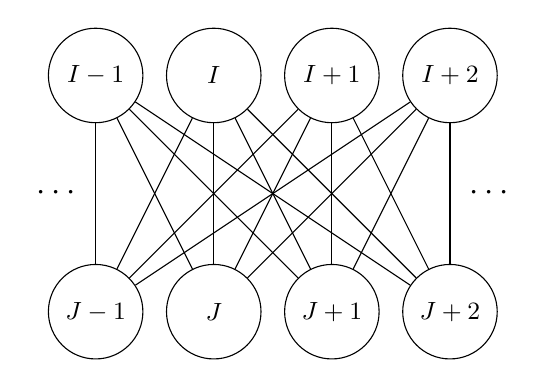
\begin{tikzpicture}[node distance={5mm}, main/.style = {draw, circle, minimum size=1.2cm}]

            \node (D0) at (-0.5,-1.5) {\large $\cdots$};
            \node (D1) at (5,-1.5) {\large $\cdots$};

            % Nodes
            \node[main] (I0) at (0,0) {\small $I-1$};
            \node[main] (I1) at (1.5,0) {\small $I$};
            \node[main] (I2) at (3,0) {\small $I+1$};
            \node[main] (I3) at (4.5,0) {\small $I+2$};
            \node[main] (J0) at (0,-3) {\small $J-1$};
            \node[main] (J1) at (1.5,-3) {\small $J$};
            \node[main] (J2) at (3,-3) {\small $J+1$};
            \node[main] (J3) at (4.5,-3) {\small $J+2$};
    
            % Edges
            \draw (I0) to (J0);
            \draw (I0) to (J1);
            \draw (I0) to (J2);
            \draw (I0) to (J3);
            \draw (I1) to (J0);
            \draw (I1) to (J1);
            \draw (I1) to (J2);
            \draw (I1) to (J3);
            \draw (I2) to (J0);
            \draw (I2) to (J1);
            \draw (I2) to (J2);
            \draw (I2) to (J3);
            \draw (I3) to (J0);
            \draw (I3) to (J1);
            \draw (I3) to (J2);
            \draw (I3) to (J3);
        \end{tikzpicture}
        \caption{Vollständig bipartiter Teilgraph zu Knoten $I \neq J$ mit nicht invertierbarem $M_{IJ}$}
        \label{fig:biclique-graph}
    \end{subfigure}
    \hfill
    \begin{subfigure}[b]{0.47\textwidth}
        \centering
        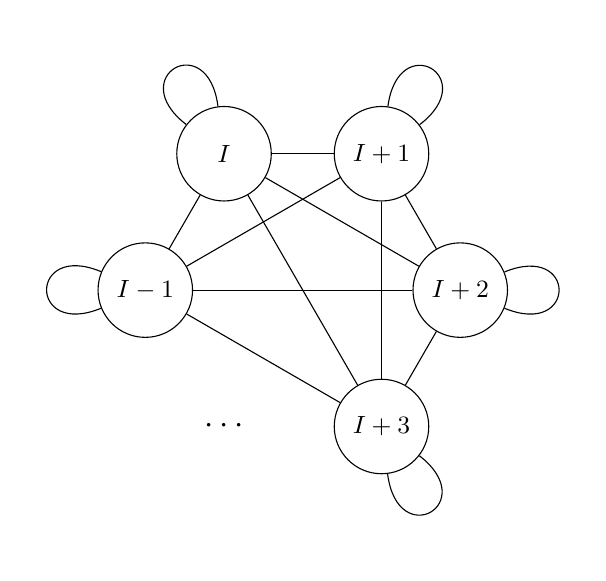
\begin{tikzpicture}[node distance={5mm}, main/.style = {draw, circle, minimum size=1.2cm}]
            % Nodes
            \node[main] (I0) at ({360/6 * 0}: 2cm) {\small $I+2$};
            \node[main] (I1) at ({360/6 * 1}: 2cm) {\small $I+1$};
            \node[main] (I2) at ({360/6 * 2}: 2cm) {\small $I$};
            \node[main] (I3) at ({360/6 * 3}: 2cm) {\small $I-1$};
            \node (D1) at ({360/6 * 4}: 2cm) {\large $\cdots$};
            \node[main] (I4) at ({360/6 * 5}: 2cm) {\small $I+3$};

            \draw (I0) to[loop, out=22.5, in=-22.5, distance=1cm] (I0);         
            \draw (I0) to (I1);
            \draw (I0) to (I2);
            \draw (I0) to (I3);
            \draw (I0) to (I4);            
            \draw (I1) to[loop, out=82.5, in=37.5, distance=1cm] (I1);            
            \draw (I1) to (I2);
            \draw (I1) to (I3);
            \draw (I1) to (I4);
            \draw (I2) to[loop, out=142.5, in=97.5, distance=1cm] (I2);    
            \draw (I2) to (I3);
            \draw (I2) to (I4);
            \draw (I3) to[loop, out=202.5, in=157.5, distance=1cm] (I3);    
            \draw (I3) to (I4);
            \draw (I4) to[loop, out=322.5, in=277.5, distance=1cm] (I4);    
        \end{tikzpicture}
        \caption{Vollständiger Teilgraph zum Knoten $I$ mit nicht invertierbarem $M_{II}$}
        \label{fig:complete-graph}
    \end{subfigure}
    \caption{Bipartite Untergraphen in $G_a$ und $G_{a^{-1}}$}
    \label{fig:subgraphs}
\end{figure}

Sei $G[V]$ der durch die Knotenmenge $V$ induzierte Teilgraph von $G$. Aus \Cref{satz:skalierung} ergeben sich weitere Symmetrien in $G_a$. Demnach sind die folgenden Aussagen äquivalent

\begin{align*}
    &(\det{} M_{I,J})(a) = 0 \\
    \iff &(\det{} M_{-I,-J})(a) = 0 \\
    \iff &(\det{} M_{-I,J})(a^{-1}) = 0 \\
    \iff &(\det{} M_{I,-J})(a^{-1}) = 0
\end{align*}


und die induzierten Teilgraphen $G_a[I \cup J]$, $G_a[-I \cup -J]$, $G_{a^{-1}}[-I \cup J]$, $G_{a^{-1}}[I \cup -J]$ isomorph.

Somit induziert die bijektive Abbildung $f:V \to V, I \mapsto -I$ einen nicht trivialen Graphautomorphismus und einen Graphisomorphismus zwischen $G_a$ und $G_{a^{-1}}$.